\documentclass[8pt]{beamer}
\usepackage{pscyr}
\usepackage[english,russian]{babel}
\usepackage[utf8]{inputenc}
\usepackage{graphicx}
\setbeamertemplate{caption}[numbered]
\usetheme{CambridgeUS}
\beamertemplatesquareitem
\begin{document}
\title{Моделирование фильтра циклон}
\author{Дмитрий Богданов}
\institute{СПБГПУ}
\date{\today}
\frame{\titlepage}
\frame{\frametitle{Содержание}\small{\tableofcontents}}
\section{Постановка задачи}

\frame{\frametitle{Геометрия фильтра}
\small{
\hspace{0.02\textwidth}
  \begin{minipage}[t]{0.5\linewidth}
  \vspace{0.2\textwidth}
    \begin{table}[h]
      \caption{Геометрия фильтра}
      \hline
      \begin{tabular}{c c}
        Диаметр цилиндра, $D$ & $0.205m$ \\
        Диаметр выходной трубы, $D_e$ & $0.5D$ \\
        Высота входного канала, $a$ & $0.5D$ \\
        Ширина входного канала, $b$ & $0.2D$ \\
        Длина выходной трубы, $h_e$ & $0.75D$ \\
        полная высота фильтра, $H$ & $4.0D$ \\
        Высота цилиндра, $h$ & $1.5D$ \\
        Диаметр нижнего сечения фильтра, $B$ & $0.36D$ \\
      \end{tabular}
    \end{table}
  \end{minipage}
  \hfill
  \begin{minipage}[t]{0.45\linewidth}
    \centering
    \vspace{-1.5ex}
    \begin{figure}
    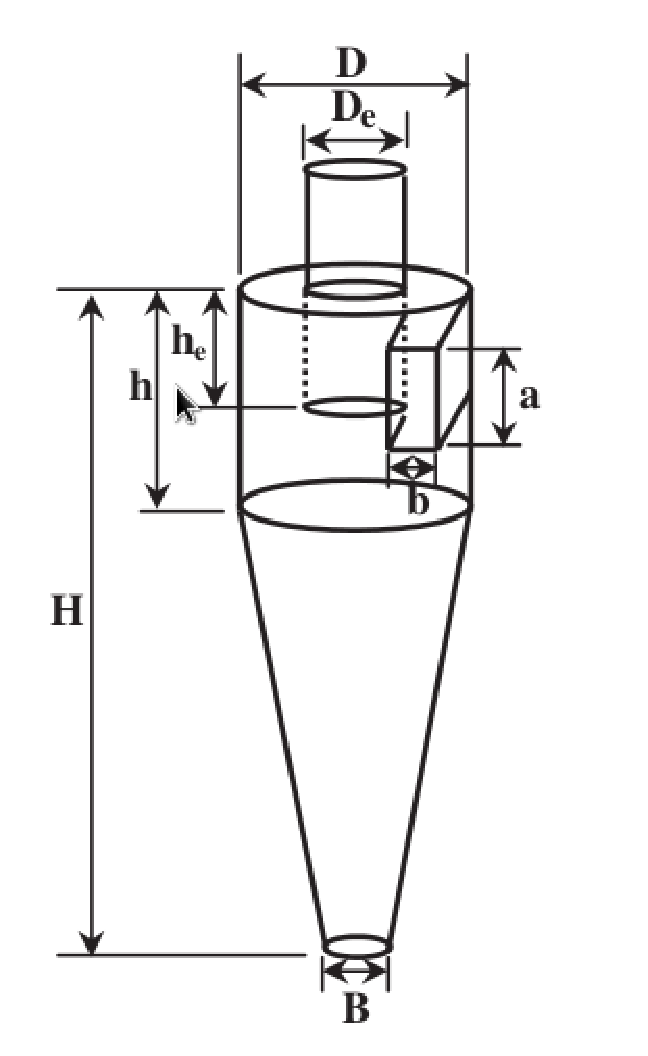
\includegraphics[scale=0.3]{Geometry}
    \caption{Схема фильтра}\label{fig:geometry}
    \end{figure}
  \end{minipage}
}
}%offrame
\section{Определяющие уравнения}
\frame{\frametitle{Уравнения движения}
\small{
  \begin{eqnarray}
    \nonumber
    \text{Уравнение неразрывности:} \\
    \frac{\partial \rho}{\partial t} + \nabla{(\rho \vec{V})}&=& 0, \\
    \hline
    \nonumber
    \\
    \nonumber
    \text{Уравнение баланса импульса:} \\
    \frac{\partial \rho \vec{V}}{\partial t} + \nabla{(\rho \vec{V} \vec{V})} &=& - \nabla{p} + (\mu + \mu_t) \nabla^2{\vec{V}} + \rho \vec{S_{V}}, \\
    \hline 
    \nonumber
    \\
    \nonumber
    \text{Уравнение баланса энергии:}\\
    \frac{\partial \rho h}{\partial t} + \nabla {(\rho \vec{V} h)} &=&  \frac{\partial p}{\partial t} + (\alpha + \alpha_t)\nabla^2{h} + \rho S_h, \quad \text{где } \alpha_t = \mu_t/Pr_t, \\
    \hline
    \nonumber
    \\
    \nonumber
    \text{Уравнение состояния:}\\
    p &=& \rho R T
  \end{eqnarray}
}
}
\frame{\frametitle{Модель турбулентности}
  \small{
    \begin{eqnarray}
      \nonumber
      \text{Уравнение переноса кинетической энергии:} \\
      \nonumber
      \\
      \frac{\partial \rho k}{\partial t} + \nabla{(\rho \vec{V} k)} = P_k f_{rot} + \beta^* \rho k \omega + \nabla{\left[(\mu + \mu_t) \nabla k\right]}, \\
      \hline
      \nonumber 
      \\
      \nonumber
      \text{Уравнение переноса удельной скорости диссипации:} \\
      \nonumber
      \\
      \frac{\partial \rho \omega}{\partial t} + \nabla{(\rho \vec{V} \omega)} = \alpha \frac{\rho P_k }{\mu_t}f_{rot} -D_{\omega} + Cd_{\omega} + \nabla{\left[(\mu + \mu_t) \nabla \omega\right]}, \\
      \hline 
      \nonumber
      \\
      \nonumber
      \text{Поправка на кривизну линий тока:}\\
      \nonumber
      \\
      \nonumber
      f_{r1}(r^*,\tilde{r}) = 2r^*\left( \frac{1+C_{r1}}{1+ r^*} \right)\left[ 1-C_{r3}\arctan{(C_{r2}\tilde{r})} \right] - C_{r1}, \\
      \tilde{r} = 2\Omega_{ik}S_{kj}\frac{DS_{ij}}{Dt}\frac{1}{\Omega D^3}, \quad D^2 = \max(S^2, 0.09 \omega^2), \\
      \nonumber
      S^2 = 2 S_{ij}S_{ij}, \quad \Omega^2 = 2 \Omega_{ij} \Omega_{ij}, \quad r^* = S/\Omega, \\
      \nonumber
      C_{r1} = 1, \quad C_{r2} = 2, \quad C_{r3} = 1, \quad f_{rot} = \max[\min(f_{r1},1.25),0]
    \end{eqnarray}
  }
}
\frame{\frametitle{Модель частиц}
  
}
\section{Верификация модели турбулентности}
\frame{\frametitle{Течение в трубе}
\tiny{
  \begin{minipage}[t]{0.5\linewidth}
    \vspace{0.2\textwidth}
    \begin{table}[h]
      \caption{Параметры задачи о течении в трубе}
      \hline
      \begin{tabular}{c c}
        Диаметр входного сечения, $D_{in}$ & $0.1 [m]$ \\
        Диаметр выходного сечения, $D_{out}$ & $0.22 [m]$ \\
        Длина трубы, $L$ & $0.55m$ \\
        Массовый расход через входное течение трубы, $Q_{in}$ & $0.08 [kg/s]$ \\
        Кинетическая энергия турбулентности на входе, $k_{in}$ & $0.00375 [m^2/s^2]$ \\
        Удельная скорость диссипации на входе, $\omega_{in}$ & $2.6 [s^{-1}]$ \\
        Угловая скорость вращения на входе, $w_{in}$ & $8000 [rad/min]$ \\
        Давление на выходном сечении, $p_{out}$ & $101325 [Pa]$ \\
        Температура во входном сечении, $T_{in}$ & $300 [K]$ \\
        Температура стенок, $T_{w}$, & $300 [K]$
      \end{tabular}
    \end{table}
  \end{minipage}
  \hspace{0.05\textwidth}
    \begin{minipage}[t]{0.35\linewidth}
    \centering
    \vspace{-1.5ex}
    \begin{figure}
    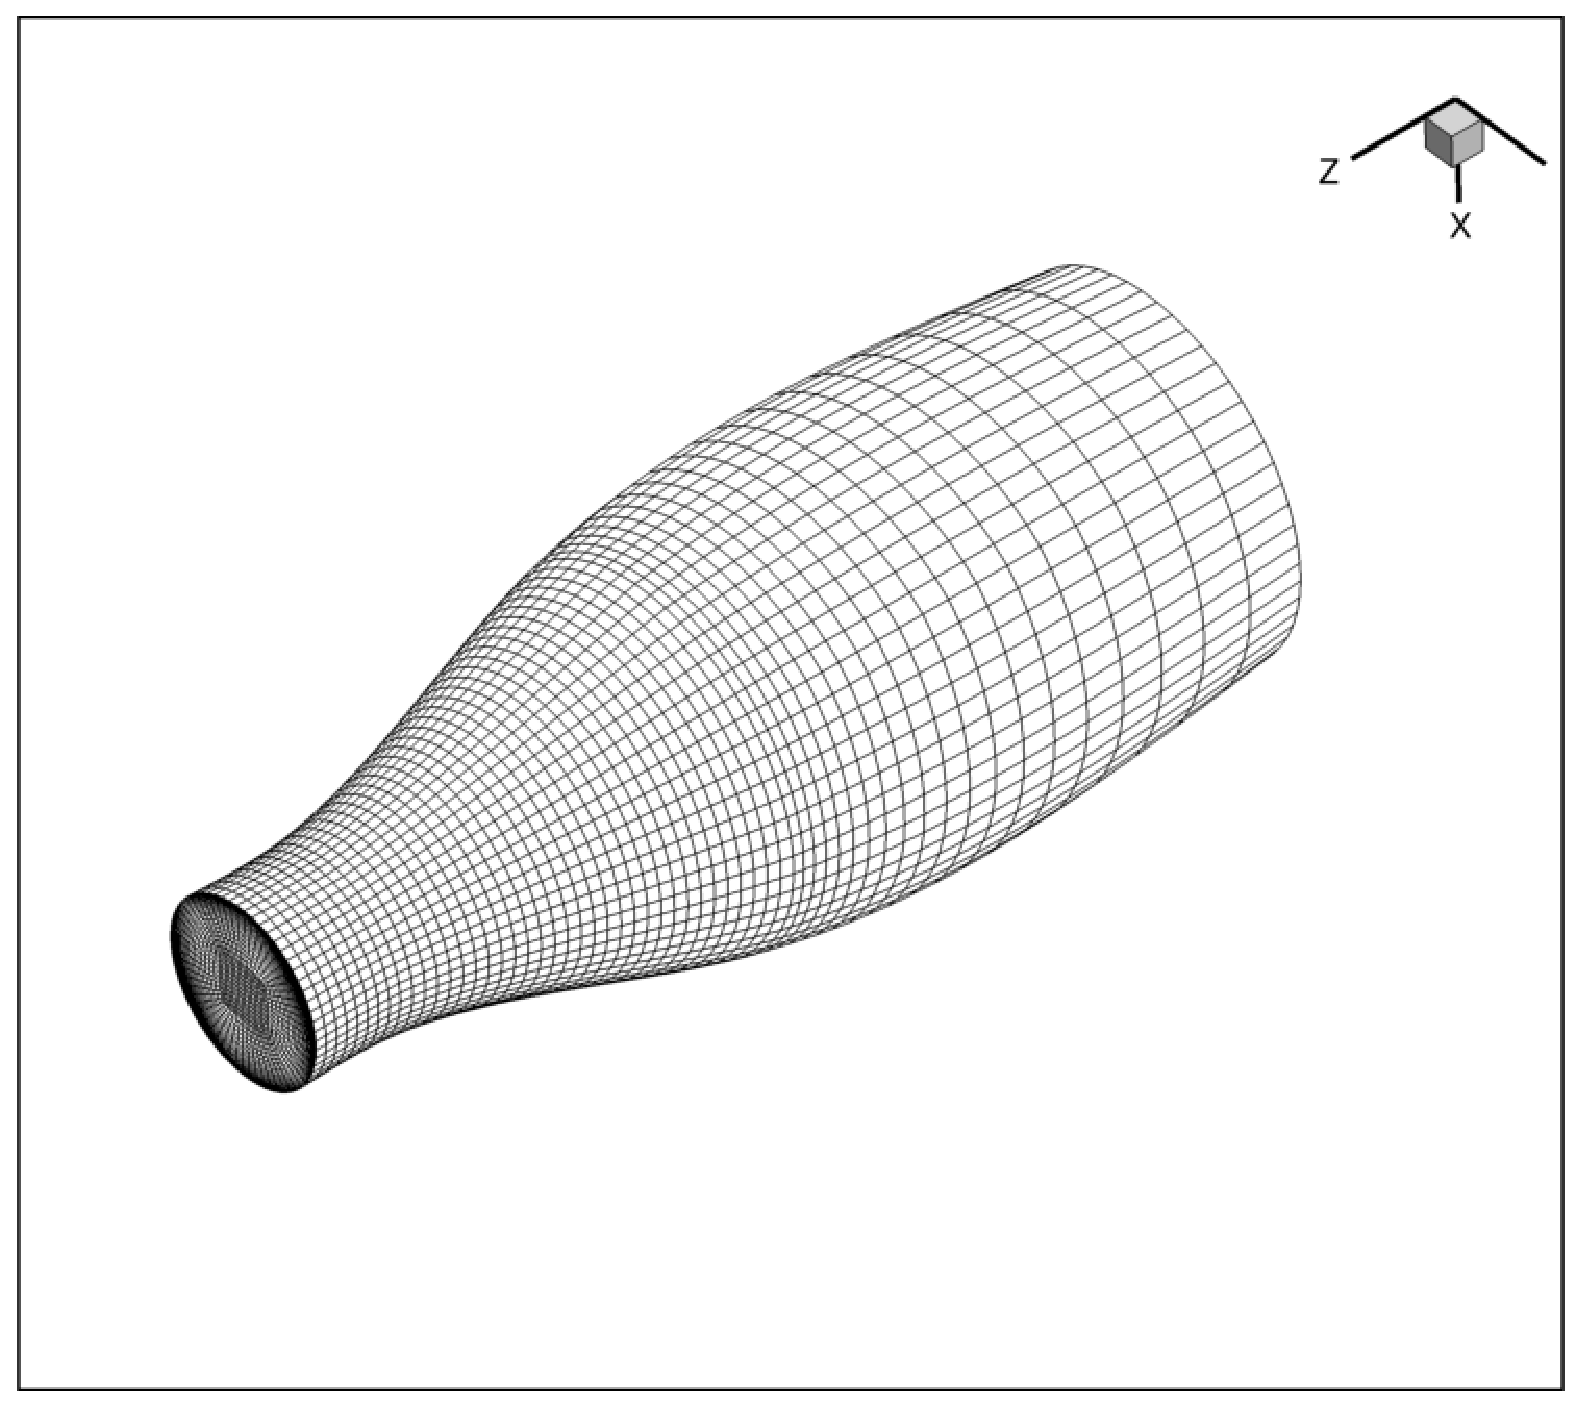
\includegraphics[scale=0.2]{swirlMesh}
    \caption{Сетка для задачи о течении в трубе}\label{fig:verify}
    \end{figure}
  \end{minipage}
  }
}
\end{document}
